\documentclass[12pt]{article}
\usepackage{dsfont}
\usepackage{textcomp}
\usepackage{amsmath}
\usepackage{graphicx}


\begin{document}


\title{Solutions to Sheet 4}
\author{Lukas Drexler, Leif Van Holland \\ \\
\textsc{Pattern Matching and Machine Learning} \\
\textsc{for Audio Signal Processing}}
\maketitle

\section*{Task 4.1}
\subsection*{(a)}
The spectrum of the noise signal is given by $\mathbf{B} = \text{DFT}_{N}\mathbf{b} = \text{DFT}_{N}(\mathbf{a} + \mathbf{r})
= \text{DFT}_{N}\mathbf{a} + \text{DFT}_{N}\mathbf{r} = \mathbf{A} + \mathbf{R}$.
We know that we can express the vector $\mathbf{a}$ in terms of the Fourier basis vectors:
\begin{align*}
\mathbf{a} = \frac{1}{2i}(\mathbf{u}_{4} - \mathbf{u}_{508})
\end{align*} 
With $\langle\mathbf{u}_{k}|\mathbf{u}_{l}\rangle = N\cdot\delta_{k,l}$, we obtain
\begin{align*}
|\hat{\mathbf{a}}(k)| = \begin{cases}
\frac{N}{2},\qquad&\text{if }k=4 \text{ or } k=508\\
0,\qquad&\text{ otherwise.}
\end{cases}
\end{align*}
So the only non-zero entries of $\mathbf{A}$ are at $k=4$ and $k=508$.  We also know that $|\mathbf{A}(k)| > 2\theta$ wherever $\mathbf{A}(k)\neq 0$, and $|\mathbf{R}(k)|\leq \theta$ for all $k \in [0:N-1]$. So we can conclude that $|\mathbf{A}+\mathbf{R}|>\theta$ for these entries, i.e. these entries are unchanged in $\mathbf{B}_{\theta}$. Also $|\mathbf{A}+\mathbf{R}|\leq \theta $ for all other entries. So $\mathbf{B}_{\theta}$ is given by
\begin{align*}
\mathbf{B}_{\theta}(k) = \begin{cases}
\mathbf{A}(k) + \mathbf{R}(k),\qquad&\text{ if }\mathbf{A}(k)\neq 0\\
0,\qquad&\text{ otherwise}.
\end{cases}
\end{align*}
Now let $\mathbf{R}_{\theta}$ be defined by
\begin{align*}
\mathbf{R}_{\theta}(k) = \begin{cases}
\mathbf{R}(k),\qquad&\text{ if }\mathbf{A}(k)\neq 0\\
0,\qquad&\text{ otherwise}.
\end{cases}
\end{align*}
Then we can write $\mathbf{B}_{\theta} = \mathbf{A} + \mathbf{R}_{\theta}$.
\subsection*{(b)}
$\tilde{\mathbf{a}} = \text{DFT}_{N}^{-1}\mathbf{B}_{\theta} = \text{DFT}_{N}^{-1}(\mathbf{A}+\mathbf{R}_{\theta}) = 
\text{DFT}_{N}^{-1}\mathbf{A} + \text{DFT}_{N}^{-1}\mathbf{R}_{\theta} = \mathbf{a} + \text{DFT}_{N}^{-1}\mathbf{R}_{\theta}$.


\section*{Task 4.2}

\begin{figure}[h]
    \centering
    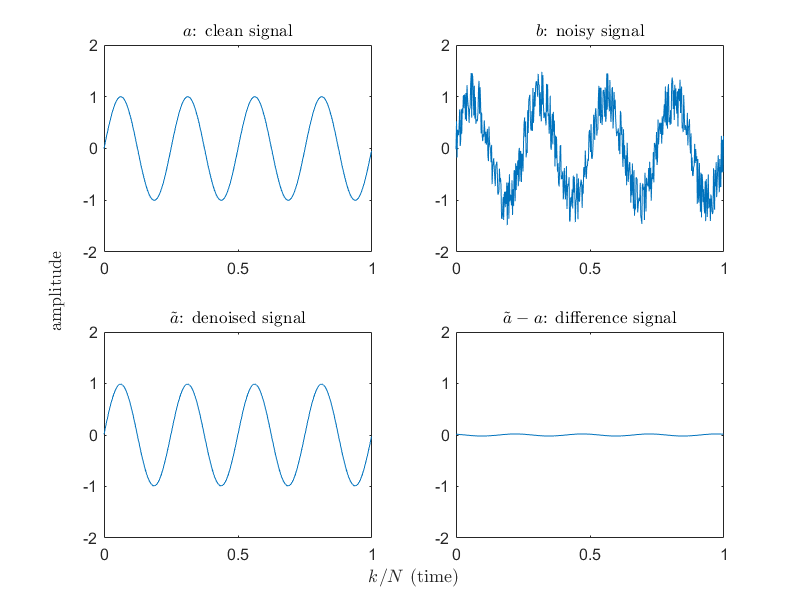
\includegraphics[width=\textwidth]{denoise.png}
    \caption{The denoising procedure applied to the signal $b$ from above.}
    \label{fig:my_label}
\end{figure}


\end{document}
